% Figure 4. Start with people who already know you. Labels: LABELS.md, Figure 4.
\def\eeprepfigure{1}
\providecommand{\eepstyledir}{../style}% repo: ../style
\input{\eepstyledir/circuitikz-preamble.tex}
% Colours, fonts, and text styles for the Get hired figures.
% Input after style/circuitikz-preamble.tex (in the repo: ../../style/circuitikz-preamble.tex).
% Define \eepdark before this file for the dark build. Same names as the resume figures,
% plus the rest of the navy palette. Crimson (eepaccent) marks one thing per figure.
\setmainfont{Newsreader}[
  BoldFont={Newsreader Bold},
  ItalicFont={Newsreader Italic},
  BoldItalicFont={Newsreader Bold Italic},
]
\usetikzlibrary{arrows.meta,calc,decorations.pathreplacing}
\ifdefined\eepdark
  \definecolor{eepink}{HTML}{ECEEF2}
  \definecolor{eeptext}{HTML}{D0D4DB}
  \definecolor{eepinktwo}{HTML}{A6AFBF}
  \definecolor{eepmute}{HTML}{8F95A0}
  \definecolor{eepsilver}{HTML}{76808F}
  \definecolor{eeprule}{HTML}{3B4352}
  \definecolor{eepwash}{HTML}{17243A}
  \definecolor{eepsunken}{HTML}{101828}
  \definecolor{eepfill}{HTML}{131C2E}
  \definecolor{eeppaper}{HTML}{0D1524}
  \definecolor{eepaccent}{HTML}{E06A5F}
  \definecolor{eepaccentsoft}{HTML}{2A1A24}
\else
  \definecolor{eepink}{HTML}{16233A}
  \definecolor{eeptext}{HTML}{232A39}
  \definecolor{eepinktwo}{HTML}{424D63}
  \definecolor{eepmute}{HTML}{5E636C}
  \definecolor{eepsilver}{HTML}{838C9A}
  \definecolor{eeprule}{HTML}{C4C8CF}
  \definecolor{eepwash}{HTML}{E7ECF3}
  \definecolor{eepsunken}{HTML}{F3F4F6}
  \definecolor{eepfill}{HTML}{FFFFFF}
  \definecolor{eeppaper}{HTML}{FBFBFC}
  \definecolor{eepaccent}{HTML}{A3201D}
  \definecolor{eepaccentsoft}{HTML}{F8ECEA}
\fi
% Draw in y-down points so coordinates read like a mockup: [x=1pt, y=-1pt].
\tikzset{
  eeptitle/.style={anchor=base west, inner sep=0pt, text=eepink, font=\rmfamily\bfseries\fontsize{26}{31}\selectfont},
  eephead/.style={inner sep=0pt, text=eepink, font=\sffamily\bfseries\fontsize{14.5}{18}\selectfont},
  eepbody/.style={inner sep=0pt, text=eepinktwo, font=\sffamily\fontsize{13}{17}\selectfont},
  eepnote/.style={inner sep=0pt, text=eepmute, font=\sffamily\fontsize{12.5}{16}\selectfont},
  eepsrc/.style={anchor=north west, inner sep=0pt, align=left, text=eepmute, font=\sffamily\fontsize{11}{14.5}\selectfont},
  eepbox/.style={draw=eepink, fill=eepfill, rounded corners=4pt},
  eepfocus/.style={draw=eepaccent, fill=eepfill, rounded corners=4pt, line width=1.8pt},
  eeparrow/.style={-{Stealth[length=8pt,width=6pt]}},
  eepdash/.style={dash pattern=on 4pt off 4pt},
  eeplead/.style={draw=eepsilver, line width=0.9pt},
}
% A dot on a trace, like a schematic junction.
\newcommand{\eepdot}[2][eepink]{\fill[#1] #2 circle (3.6pt);}
% Short labels never hyphenate.
\hyphenpenalty=10000 \exhyphenpenalty=10000
% One space after a full stop, as on the site.
\frenchspacing

\begin{document}
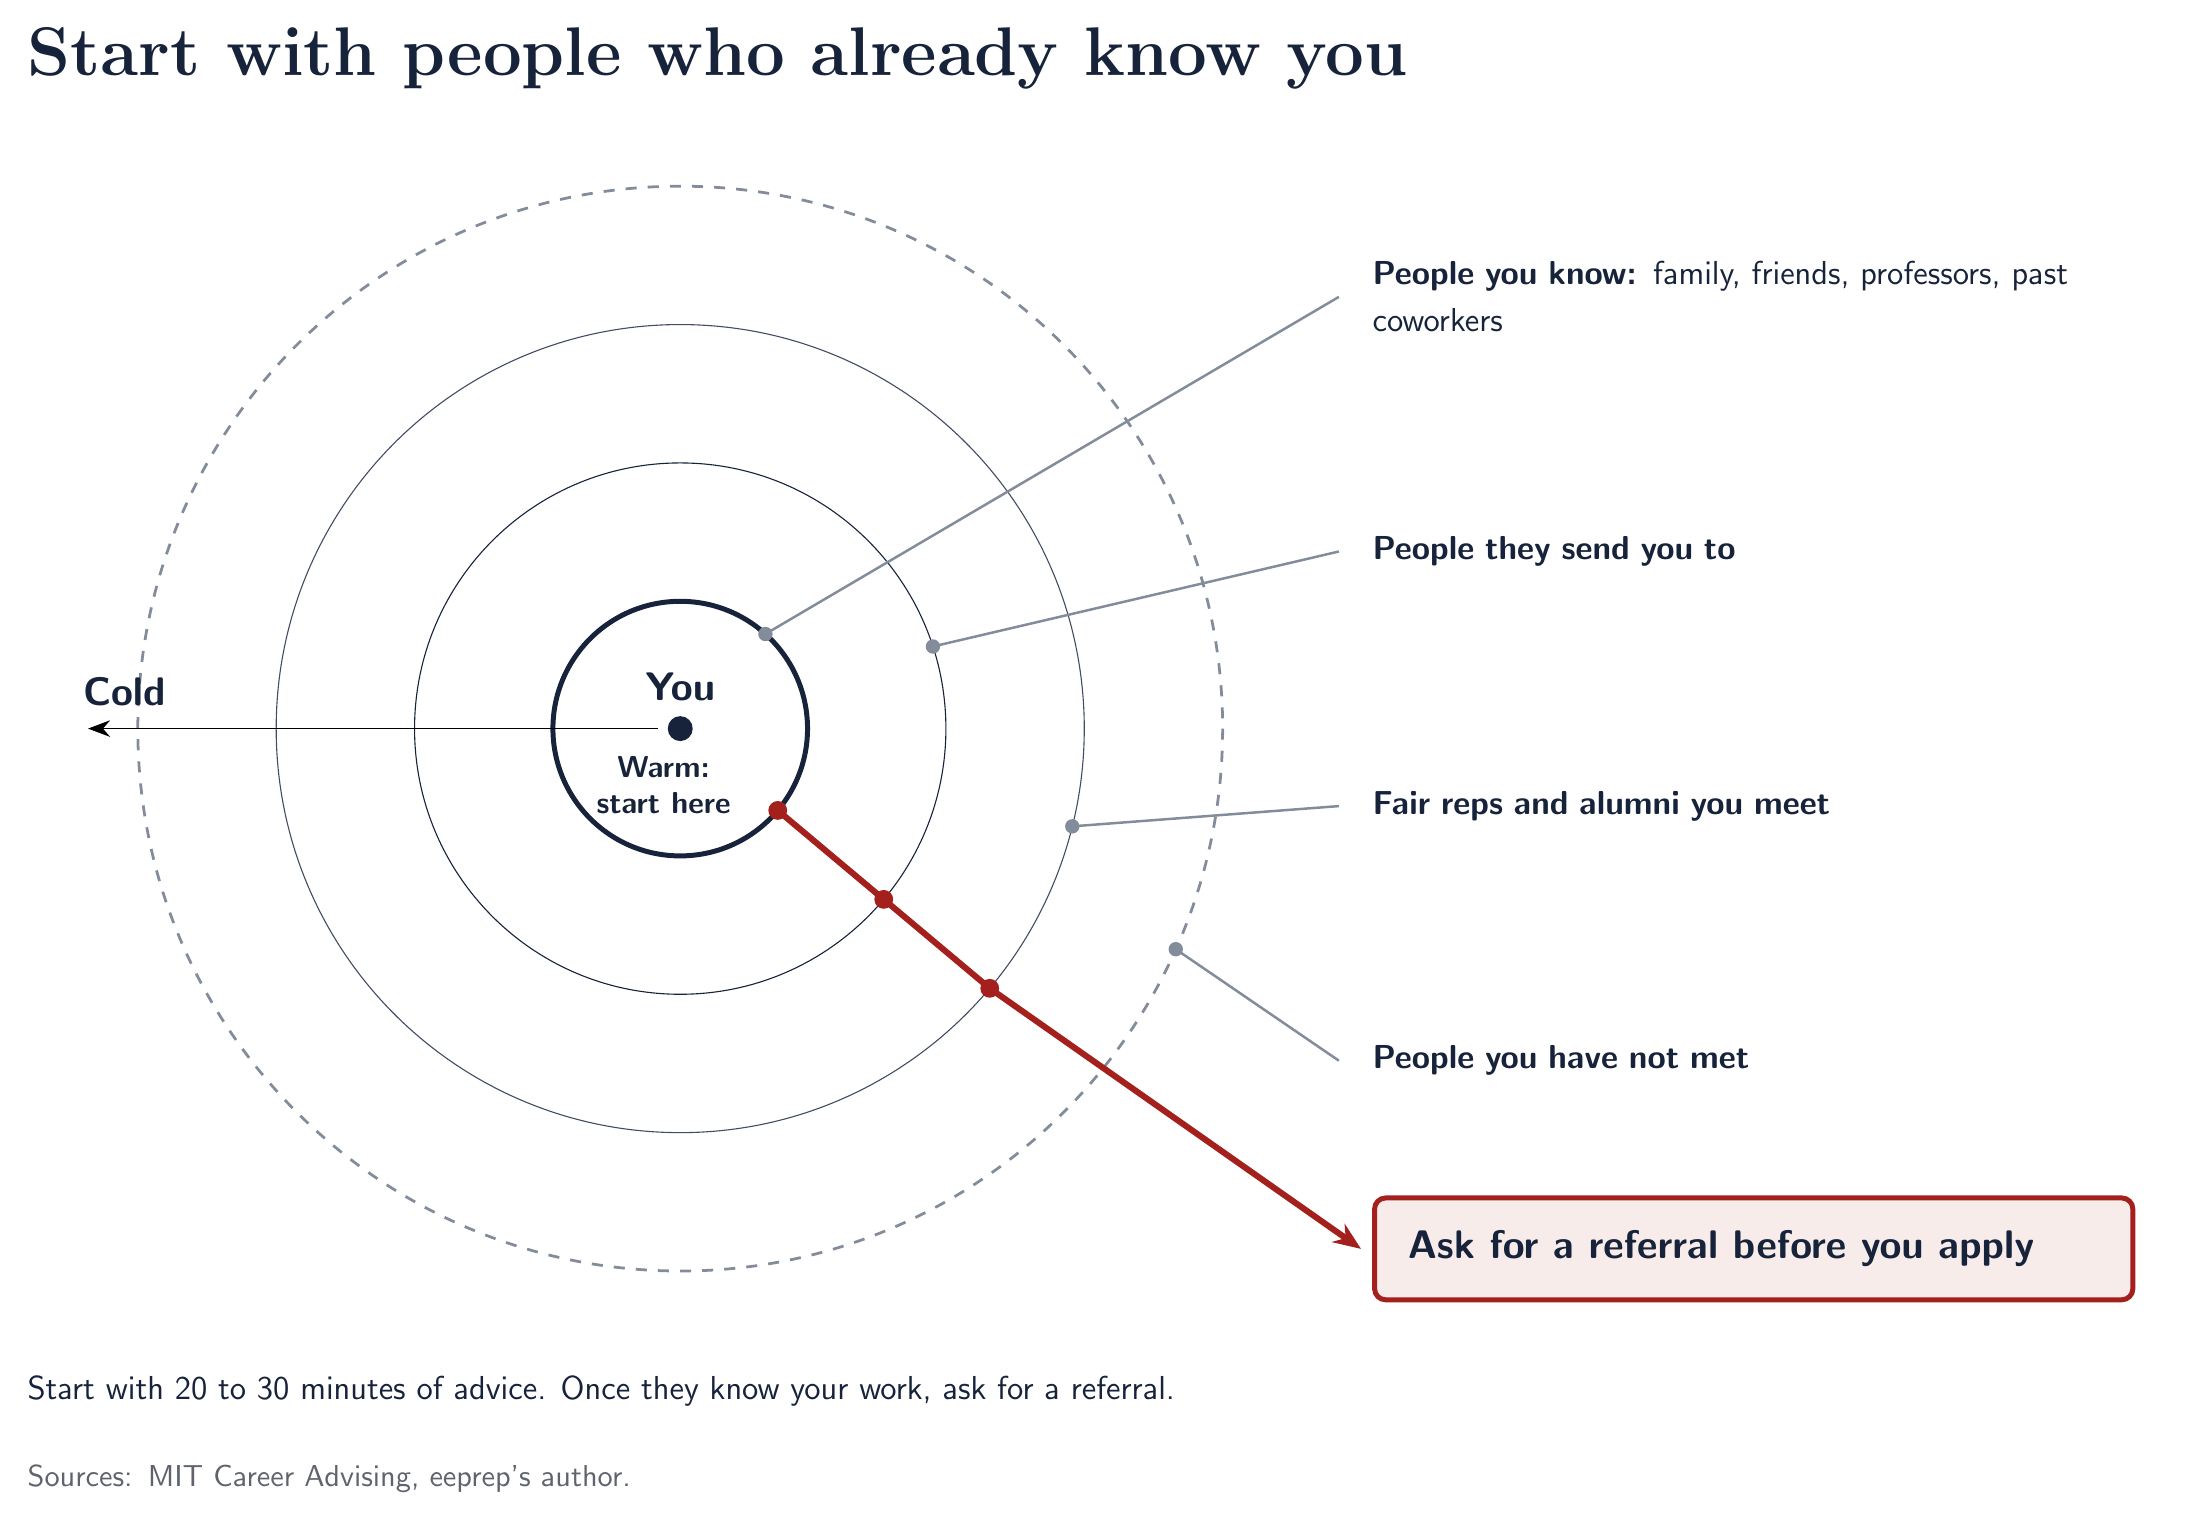
\begin{tikzpicture}[x=1pt,y=-1pt]
  \def\cx{236}\def\cy{266}
  \node[eeptitle] at (0,30) {Start with people who already know you};
  % Four rings, warm inside to cold outside.
  \draw[eepsilver, line width=1pt, eepdash] (\cx,\cy) circle (196);
  \draw[eepinktwo] (\cx,\cy) circle (146);
  \draw[eepink] (\cx,\cy) circle (96);
  \draw[eepink, line width=1.8pt] (\cx,\cy) circle (46);
  % The one arrow: from the centre outward.
  \draw[eeparrow] (\cx-8,\cy) -- (\cx-214,\cy);
  \node[eephead, anchor=south west] at (\cx-216,\cy-8) {Cold};
  \fill[eepink] (\cx,\cy) circle (4.5pt);
  \node[eephead, anchor=south] at (\cx,\cy-10) {You};
  \node[anchor=north, align=center, inner sep=0pt, text=eepink, font=\sffamily\bfseries\fontsize{11}{13}\selectfont] at (\cx-6,\cy+10) {Warm:\\start here};
  % Leaders to the labels.
  \def\lx{486}
  \foreach \r/\a/\ly in {46/-48/110, 96/-18/202, 146/14/294, 196/24/386} {
    \draw[eeplead] ({\cx+\r*cos(\a)},{\cy+\r*sin(\a)}) -- (\lx-12,\ly);
    \fill[eepsilver] ({\cx+\r*cos(\a)},{\cy+\r*sin(\a)}) circle (2.6pt);
  }
  \node[eepbody, text=eepink, anchor=west, text width=280pt, align=left] at (\lx,110) {\textbf{People you know:} family, friends, professors, past coworkers};
  \node[eepbody, text=eepink, anchor=west, text width=280pt, align=left] at (\lx,202) {\textbf{People they send you to}};
  \node[eepbody, text=eepink, anchor=west, text width=280pt, align=left] at (\lx,294) {\textbf{Fair reps and alumni you meet}};
  \node[eepbody, text=eepink, anchor=west, text width=280pt, align=left] at (\lx,386) {\textbf{People you have not met}};
  % The referral arrow (crimson): from rings 1 to 3 out to a box.
  \foreach \r in {46,96,146} \fill[eepaccent] ({\cx+\r*cos(40)},{\cy+\r*sin(40)}) circle (3.4pt);
  \draw[eepaccent, line width=2.2pt] ({\cx+46*cos(40)},{\cy+46*sin(40)}) -- ({\cx+146*cos(40)},{\cy+146*sin(40)});
  \draw[eepaccent, line width=2.2pt, -{Stealth[length=10pt,width=8pt]}] ({\cx+146*cos(40)},{\cy+146*sin(40)}) -- (482,454);
  \node[draw=eepaccent, line width=1.8pt, fill=eepaccentsoft, rounded corners=4pt, eephead, text width=250pt, align=left, inner sep=12pt, anchor=west] at (486,454) {Ask for a referral before you apply};
  \node[eepbody, text=eepink, anchor=north west] at (0,500) {Start with 20 to 30 minutes of advice. Once they know your work, ask for a referral.};
  \node[eepsrc, text width=770pt] at (0,532) {Sources: MIT Career Advising, eeprep's author.};
\end{tikzpicture}
\end{document}
